% Options for packages loaded elsewhere
\PassOptionsToPackage{unicode}{hyperref}
\PassOptionsToPackage{hyphens}{url}
\PassOptionsToPackage{dvipsnames,svgnames,x11names}{xcolor}
%
\documentclass[
  letterpaper,
  DIV=11,
  numbers=noendperiod,
  twocolumn]{scrartcl}

\usepackage{amsmath,amssymb}
\usepackage{iftex}
\ifPDFTeX
  \usepackage[T1]{fontenc}
  \usepackage[utf8]{inputenc}
  \usepackage{textcomp} % provide euro and other symbols
\else % if luatex or xetex
  \usepackage{unicode-math}
  \defaultfontfeatures{Scale=MatchLowercase}
  \defaultfontfeatures[\rmfamily]{Ligatures=TeX,Scale=1}
\fi
\usepackage{lmodern}
\ifPDFTeX\else  
    % xetex/luatex font selection
\fi
% Use upquote if available, for straight quotes in verbatim environments
\IfFileExists{upquote.sty}{\usepackage{upquote}}{}
\IfFileExists{microtype.sty}{% use microtype if available
  \usepackage[]{microtype}
  \UseMicrotypeSet[protrusion]{basicmath} % disable protrusion for tt fonts
}{}
\makeatletter
\@ifundefined{KOMAClassName}{% if non-KOMA class
  \IfFileExists{parskip.sty}{%
    \usepackage{parskip}
  }{% else
    \setlength{\parindent}{0pt}
    \setlength{\parskip}{6pt plus 2pt minus 1pt}}
}{% if KOMA class
  \KOMAoptions{parskip=half}}
\makeatother
\usepackage{xcolor}
\usepackage[top=20mm,left=20mm,right=20mm,heightrounded]{geometry}
\setlength{\emergencystretch}{3em} % prevent overfull lines
\setcounter{secnumdepth}{-\maxdimen} % remove section numbering
% Make \paragraph and \subparagraph free-standing
\ifx\paragraph\undefined\else
  \let\oldparagraph\paragraph
  \renewcommand{\paragraph}[1]{\oldparagraph{#1}\mbox{}}
\fi
\ifx\subparagraph\undefined\else
  \let\oldsubparagraph\subparagraph
  \renewcommand{\subparagraph}[1]{\oldsubparagraph{#1}\mbox{}}
\fi


\providecommand{\tightlist}{%
  \setlength{\itemsep}{0pt}\setlength{\parskip}{0pt}}\usepackage{longtable,booktabs,array}
\usepackage{calc} % for calculating minipage widths
% Correct order of tables after \paragraph or \subparagraph
\usepackage{etoolbox}
\makeatletter
\patchcmd\longtable{\par}{\if@noskipsec\mbox{}\fi\par}{}{}
\makeatother
% Allow footnotes in longtable head/foot
\IfFileExists{footnotehyper.sty}{\usepackage{footnotehyper}}{\usepackage{footnote}}
\makesavenoteenv{longtable}
\usepackage{graphicx}
\makeatletter
\def\maxwidth{\ifdim\Gin@nat@width>\linewidth\linewidth\else\Gin@nat@width\fi}
\def\maxheight{\ifdim\Gin@nat@height>\textheight\textheight\else\Gin@nat@height\fi}
\makeatother
% Scale images if necessary, so that they will not overflow the page
% margins by default, and it is still possible to overwrite the defaults
% using explicit options in \includegraphics[width, height, ...]{}
\setkeys{Gin}{width=\maxwidth,height=\maxheight,keepaspectratio}
% Set default figure placement to htbp
\makeatletter
\def\fps@figure{htbp}
\makeatother

\usepackage{amsmath}
\KOMAoption{captions}{tablesignature}
\makeatletter
\makeatother
\makeatletter
\makeatother
\makeatletter
\@ifpackageloaded{caption}{}{\usepackage{caption}}
\AtBeginDocument{%
\ifdefined\contentsname
  \renewcommand*\contentsname{Table of contents}
\else
  \newcommand\contentsname{Table of contents}
\fi
\ifdefined\listfigurename
  \renewcommand*\listfigurename{List of Figures}
\else
  \newcommand\listfigurename{List of Figures}
\fi
\ifdefined\listtablename
  \renewcommand*\listtablename{List of Tables}
\else
  \newcommand\listtablename{List of Tables}
\fi
\ifdefined\figurename
  \renewcommand*\figurename{Figura}
\else
  \newcommand\figurename{Figura}
\fi
\ifdefined\tablename
  \renewcommand*\tablename{Tabla}
\else
  \newcommand\tablename{Tabla}
\fi
}
\@ifpackageloaded{float}{}{\usepackage{float}}
\floatstyle{ruled}
\@ifundefined{c@chapter}{\newfloat{codelisting}{h}{lop}}{\newfloat{codelisting}{h}{lop}[chapter]}
\floatname{codelisting}{Listing}
\newcommand*\listoflistings{\listof{codelisting}{List of Listings}}
\makeatother
\makeatletter
\@ifpackageloaded{caption}{}{\usepackage{caption}}
\@ifpackageloaded{subcaption}{}{\usepackage{subcaption}}
\makeatother
\makeatletter
\@ifpackageloaded{tcolorbox}{}{\usepackage[skins,breakable]{tcolorbox}}
\makeatother
\makeatletter
\@ifundefined{shadecolor}{\definecolor{shadecolor}{rgb}{.97, .97, .97}}
\makeatother
\makeatletter
\makeatother
\makeatletter
\makeatother
\ifLuaTeX
  \usepackage{selnolig}  % disable illegal ligatures
\fi
\IfFileExists{bookmark.sty}{\usepackage{bookmark}}{\usepackage{hyperref}}
\IfFileExists{xurl.sty}{\usepackage{xurl}}{} % add URL line breaks if available
\urlstyle{same} % disable monospaced font for URLs
\hypersetup{
  pdftitle={Tarea 2},
  pdfauthor={Sebastián Celaya; Camila Echeverría; Francisca Vilca},
  colorlinks=true,
  linkcolor={blue},
  filecolor={Maroon},
  citecolor={Blue},
  urlcolor={Blue},
  pdfcreator={LaTeX via pandoc}}

\title{Tarea 2}
\usepackage{etoolbox}
\makeatletter
\providecommand{\subtitle}[1]{% add subtitle to \maketitle
  \apptocmd{\@title}{\par {\large #1 \par}}{}{}
}
\makeatother
\subtitle{EYP3907 - Series de Tiempo}
\author{Sebastián Celaya \and Camila Echeverría \and Francisca Vilca}
\date{}

\begin{document}
\maketitle
\ifdefined\Shaded\renewenvironment{Shaded}{\begin{tcolorbox}[breakable, sharp corners, frame hidden, boxrule=0pt, interior hidden, enhanced, borderline west={3pt}{0pt}{shadecolor}]}{\end{tcolorbox}}\fi

\hypertarget{introducciuxf3n}{%
\subsection{Introducción}\label{introducciuxf3n}}

Utilizando una base de datos que contiene información sobre el ancho de
los anillos de árboles pertenecientes a la especie \emph{Pino
Silvestre}, que puede encontrarse en el siguiente
\href{https://www.ncei.noaa.gov/pub/data/paleo/treering/measurements/europe/norw001x-rwl-noaa.txt}{link},
ajustaremos un modelo ARMA y realizaremos diversos procedimientos para
comprobar su ajuste.

\hypertarget{anuxe1lisis-exploratorio}{%
\subsection{Análisis exploratorio}\label{anuxe1lisis-exploratorio}}

La figura~\ref{fig-exp1} muestra los valores del ancho del anillo
registrados entre los años 1721 y 1889.

\begin{figure}[H]

{\centering 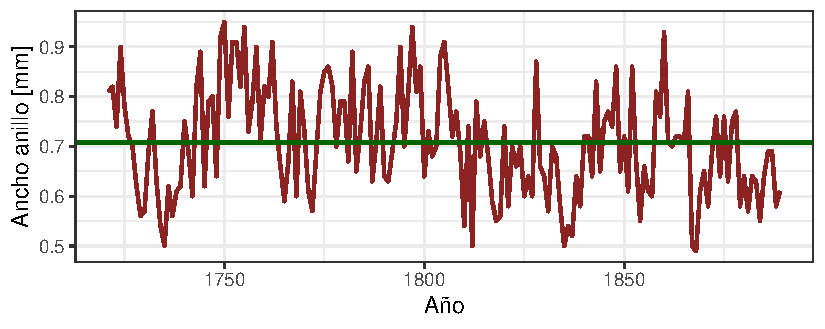
\includegraphics{pdf_tarea2_files/figure-pdf/fig-exp1-1.pdf}

}

\caption{\label{fig-exp1}Variación del ancho del anillo}

\end{figure}

Gracias a la figura~\ref{fig-exp2}, es posible ver que la mediana de
estos datos se encuentra cercana a 0.7 y que no tenemos datos atípicos,
aunque la segunda mitad de las observaciones parecieran estar
ligeramente más dispersa que la primera.

Luego, en los gráficos de la figura~\ref{fig-exp3} y la
figura~\ref{fig-exp4} podemos ver la estructura de correlación de los
datos. Si bien no se puede detectar estacionalidad a simple vista, las
observaciones sí presentan altos niveles de correlación.

\begin{figure}[H]

{\centering 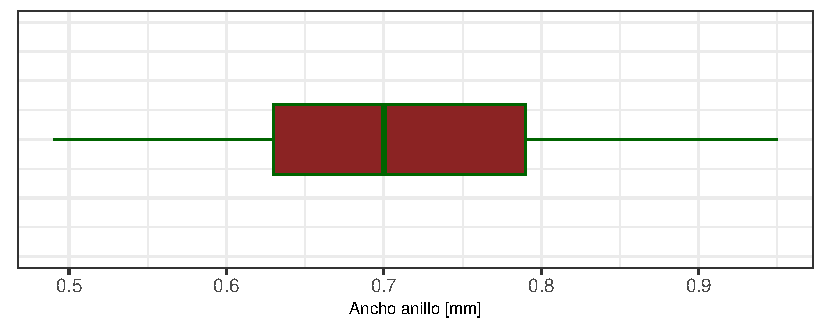
\includegraphics{pdf_tarea2_files/figure-pdf/fig-exp2-1.pdf}

}

\caption{\label{fig-exp2}Boxplot de ancho de anillo}

\end{figure}

\begin{figure}[H]

{\centering 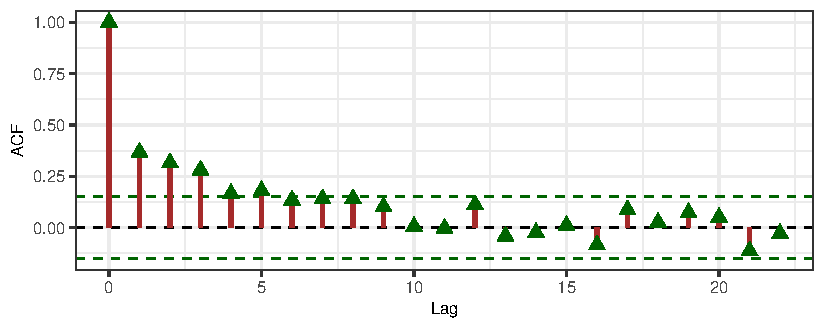
\includegraphics{pdf_tarea2_files/figure-pdf/fig-exp3-1.pdf}

}

\caption{\label{fig-exp3}Gráfico de Autocorrelación}

\end{figure}

\begin{figure}[H]

{\centering 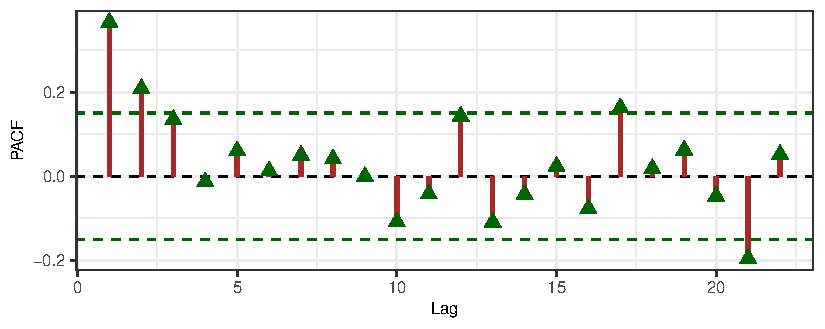
\includegraphics{pdf_tarea2_files/figure-pdf/fig-exp4-1.pdf}

}

\caption{\label{fig-exp4}Gráfico de Autocorrelación Parcial}

\end{figure}

\hypertarget{ajuste-de-un-modelo-arma}{%
\subsection{Ajuste de un modelo ARMA}\label{ajuste-de-un-modelo-arma}}

A simple vista, de los gráficos de ACF y PACF, vemos que nuestro modelo
tiene estructura de un ARMA. Por lo que, ayudándonos de la función
\texttt{auto.arima()} nuestra propuesta es un modelo arma(1,1), para que
este sea capaz de capturar toda la estructura de la serie temporal. El
modelo ajustado no considera diferenciación pues, como veremos más
adelante, la serie no es estacional.

\hypertarget{a-significancia-estaduxedstica-de-los-coeficientes-del-modelo}{%
\subsubsection{a) Significancia estadística de los coeficientes del
modelo}\label{a-significancia-estaduxedstica-de-los-coeficientes-del-modelo}}

Al revisar el valor-p asociado a cada coeficiente del modelo, es claro
notar que todos son significativos, tal como se muestra en la Tabla 1:

\begin{table}[H]
  \centering
  \caption{Resumen de estimaciones}
  \begin{tabular}{lccc}
    \toprule
     & Estimation & Stand. E & p-value \\
    \midrule
    ar1        & 0.8367     & 0.0816         & 0.0000 \\
    ma1        & -0.5698    & 0.1209         & 0.0000 \\
    intercept  & 0.7079     & 0.0196         & 0.0000 \\
    \bottomrule
  \end{tabular}
  
\end{table}

\hypertarget{b-estacionaridad-e-invertibilidad-del-modelo-arma}{%
\subsubsection{b) Estacionaridad e invertibilidad del modelo
ARMA}\label{b-estacionaridad-e-invertibilidad-del-modelo-arma}}

Una forma sencilla de comprobar la estacionalidad en los datos es con el
test de Dickey-Fuller, el cual nos da un valor-p de 0.01 que rechaza la
hipótesis nula de que los datos son estacionales. Por otro lado, una
forma sencilla de verificar invertibilidad del modelo ARMA(1,1), es de
forma gráfica, comprobando que los coeficientes se encuentren al
interior de la circunferencia unitaria, lo que puede ser apreciado en la
figura~\ref{fig-exp5}:

\begin{figure}[H]

{\centering 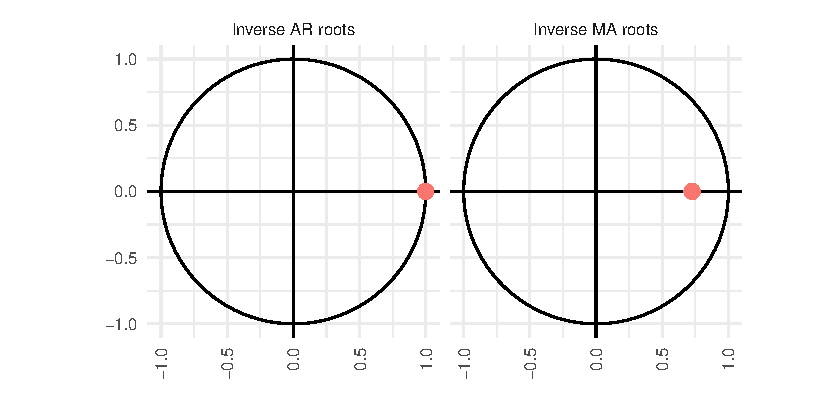
\includegraphics{pdf_tarea2_files/figure-pdf/fig-exp5-1.pdf}

}

\caption{\label{fig-exp5}Gráfico de raíces unitarias}

\end{figure}

\hypertarget{c-test-de-blancura---homocedasticidad-y-normalidad-de-los-residuos}{%
\subsubsection{c) Test de blancura - homocedasticidad y normalidad de
los
residuos}\label{c-test-de-blancura---homocedasticidad-y-normalidad-de-los-residuos}}

Los residuos del modelo deben cumplir estas propiedades. Para ello
veremos diferentes test que se le pueden aplicar para comprobar ello:

\begin{itemize}
\tightlist
\item
  La figura~\ref{fig-exp6} nos muestra que los residuos efectivamente
  corresponden a ruido blanco, es decir, no están correlacionados.
\end{itemize}

\begin{figure}[H]

{\centering 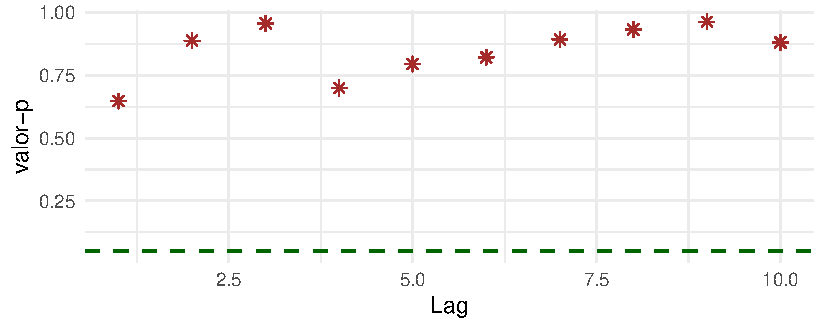
\includegraphics{pdf_tarea2_files/figure-pdf/fig-exp6-1.pdf}

}

\caption{\label{fig-exp6}Gráfico de valores-p para el estadístico
Ljung-Box}

\end{figure}

\begin{itemize}
\tightlist
\item
  Luego, al realizar el test de Kolmogorov-Smirnov para evaluar la
  normalidad, el valor-p obtenido es de 0.27 aproximadamente, por lo que
  no se rechaza la hipótesis nula: los residuos provienen de una
  distribución normal. Este ajuste se puede observar en la
  figura~\ref{fig-exp7}
\end{itemize}

\begin{figure}[H]

{\centering 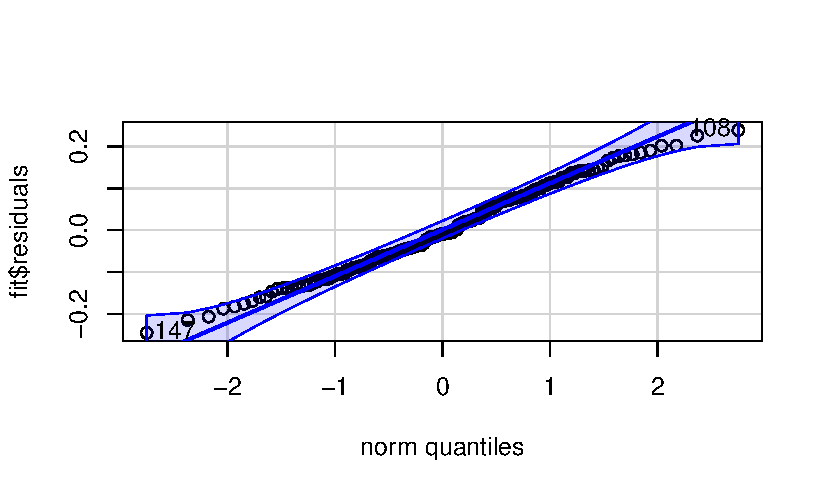
\includegraphics{pdf_tarea2_files/figure-pdf/fig-exp7-1.pdf}

}

\caption{\label{fig-exp7}Normalidad de los residuos}

\end{figure}

-De la misma manera, se obtiene un valor-p de 0.24 al realizar el test
Breusch-Pagan para evaluar homocedasticidad, por lo que podemos concluir
a favor de esta.

\hypertarget{d-es-necesario-realizar-una-transformaciuxf3n-de-box-cox}{%
\subsubsection{d) ¿Es necesario realizar una transformación de
Box-Cox?}\label{d-es-necesario-realizar-una-transformaciuxf3n-de-box-cox}}

Tras visualizar el gráfico de Box Ljung de figura~\ref{fig-exp6} se
observa que \emph{no} es necesario realizar una transformación de
Box-Cox. Además si comparamos un modelo con y sin la transformación
Box-Cox se puede observar que por AIC y BIC el mejor modelo es el modelo
sin la transformación de Box-Cox, como se logra visualizar en Tabla 2

\begin{table}[H]
  \centering
  \caption{Comparación modelos}
  \begin{tabular}{lcc}
    \toprule
    Modelo & AIC & BIC \\
    \midrule
    Sin Box-Cox & -294.0414 & -281.5218 \\
    Con Box-Cox & -128.8216 & -116.302  \\
    \bottomrule
  \end{tabular}
  
\end{table}

\hypertarget{predicciones}{%
\section{Predicciones}\label{predicciones}}

\hypertarget{a-predicciones-a-un-paso-por-el-algoritmo-durbin-levinson}{%
\subsubsection{a) Predicciones a un paso por el algoritmo
Durbin-Levinson}\label{a-predicciones-a-un-paso-por-el-algoritmo-durbin-levinson}}

Tras haber ajustado un modelo ARMA(1, 1) se generaron predicciones del
modelo.

\begin{figure}[H]

{\centering 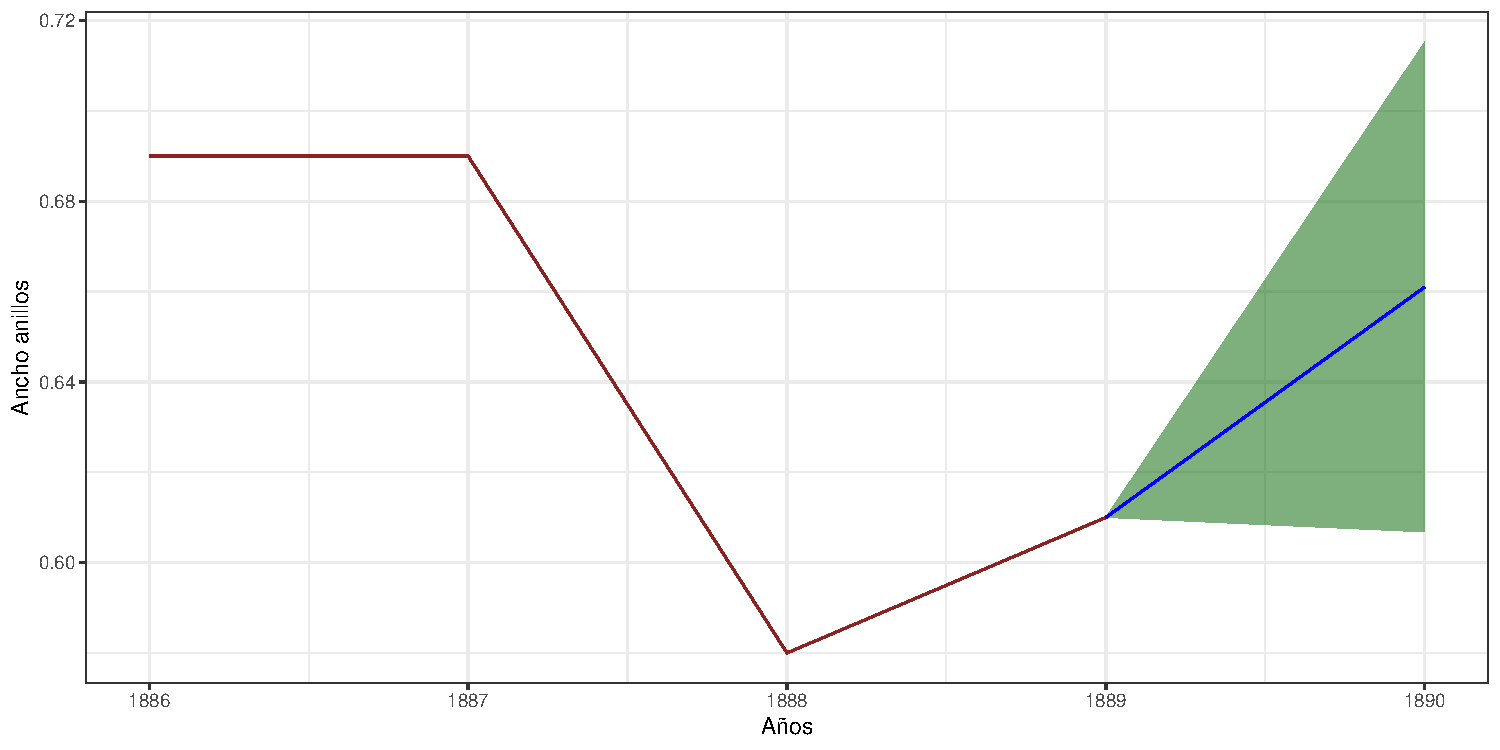
\includegraphics{pdf_tarea2_files/figure-pdf/fig-exp8-1.pdf}

}

\caption{\label{fig-exp8}Predicción a un paso por Durbin-Levinson}

\end{figure}

\begin{table}[H]
  \centering
  \caption{Predicción a un paso Durbin-Levinson}
  \begin{tabular}{lcc}
    \toprule
    Estimación Puntual & IC superior & IC inferior \\
    \midrule
    0.6610108 & 0.7152417 & 0.60678 \\
    \bottomrule
  \end{tabular}
  
\end{table}

\hypertarget{acf-empuxedrico-vs-teuxf3rico}{%
\subsubsection{ACF empírico vs
teórico}\label{acf-empuxedrico-vs-teuxf3rico}}

Calculando el ACF de un ARMA(1, 1) y generando bandas de confianza
utilizando el método Bartlett se generó el INSERTAR NUMERO DEL GRÁFICO.
El análisis del ACF revela notables similitudes entre las
autocorrelaciones empíricas y el patrón característico de un modelo ARMA
(1,1) expuesto en INSERTAR NUMERO DE LA FIGURA.

\begin{figure}[H]

{\centering 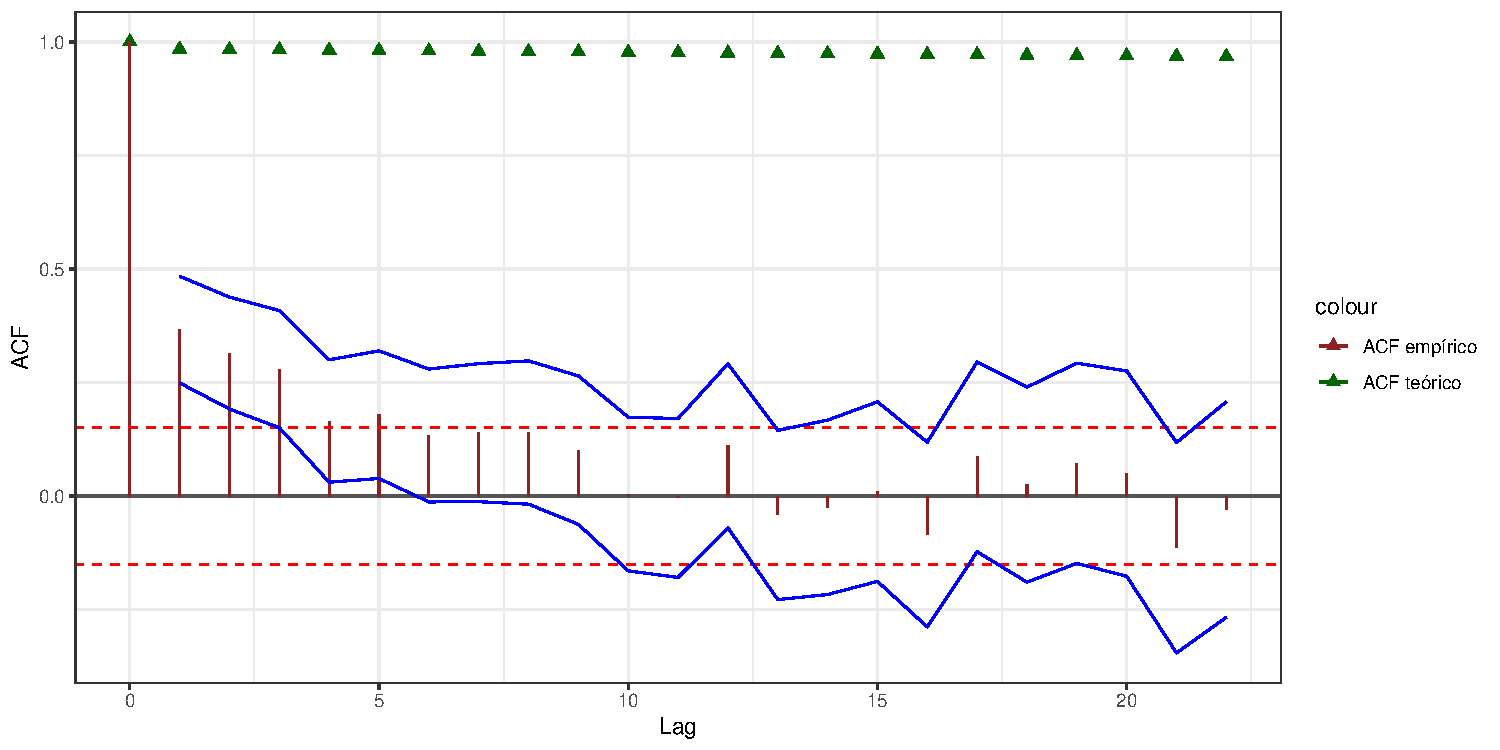
\includegraphics{pdf_tarea2_files/figure-pdf/fig-exp9-1.pdf}

}

\caption{\label{fig-exp9}ACF empírico vs teórico}

\end{figure}

\hypertarget{periodograma-vs-densidad-espectral}{%
\subsubsection{Periodograma vs Densidad
espectral}\label{periodograma-vs-densidad-espectral}}

Durante la evaluación de nuestro modelo ARMA(1,1) en las series
temporales, hemos observado una notable afinidad entre las
características espectrales previstas por el modelo y la estructura
evidente en el Periodograma como se muestra en INSERTAR NUMERO DEL
GRÁFICO. Los picos de frecuencia destacados en la Densidad Espectral del
modelo revelan una similitud con las elevaciones observadas en el
Periodograma, indicando una alineación espectral acorde entre las
predicciones del ARMA(1,1) y las características temporales de los datos
\emph{(acortable a indicando un parecido entre las predicciones del
ARMA(1,1) y los datos temporales)}.

Esta relación robusta respalda el uso del modelo ARMA(1,1) para capturar
eficazmente las componentes temporales en nuestras series temporales. La
convergencia entre la Densidad Espectral y el Periodograma demuestra la
capacidad del modelo para reflejar fielmente la variabilidad en los
datos, proporcionando una valiosa herramienta para el análisis y la
interpretación de la dinámica temporal.

\begin{figure}[H]

{\centering 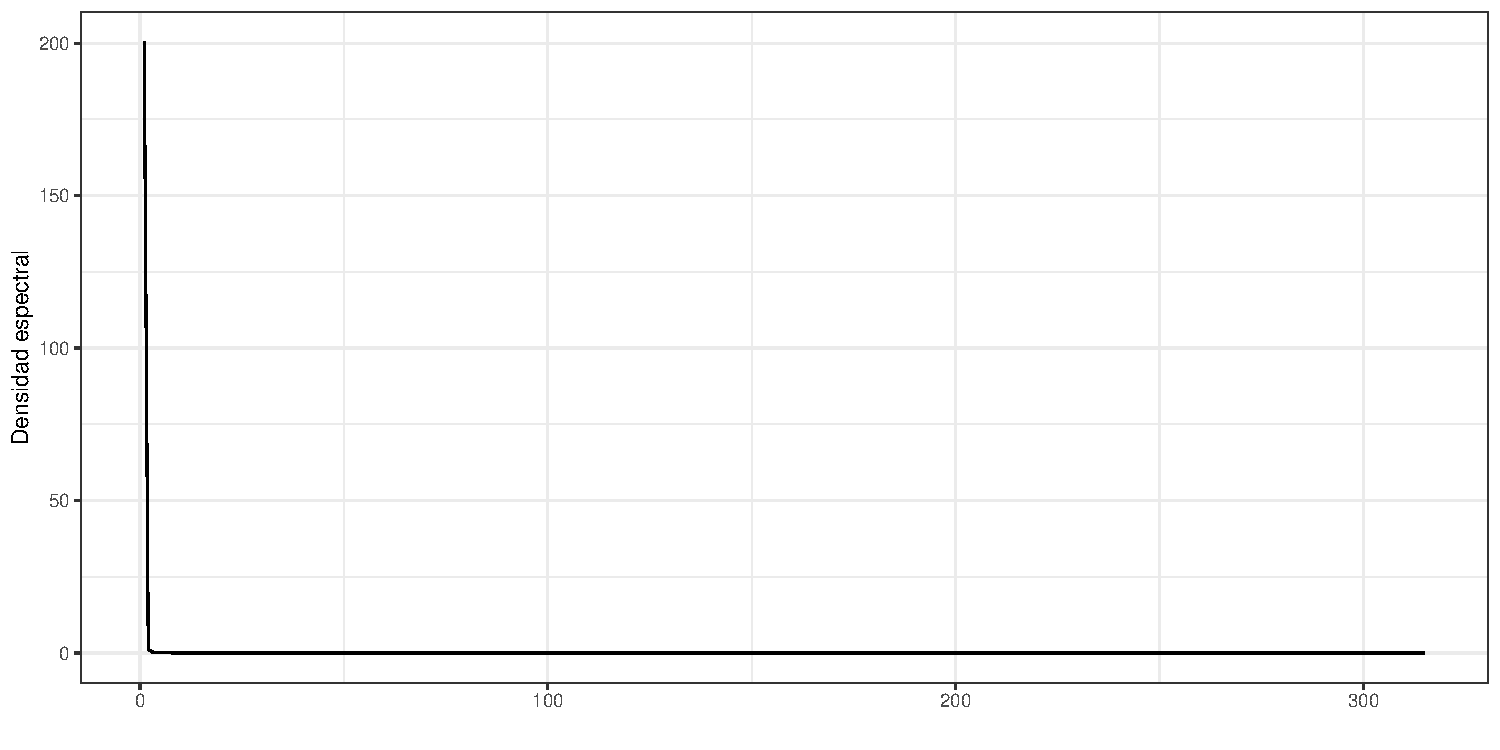
\includegraphics{pdf_tarea2_files/figure-pdf/fig-exp10-1.pdf}

}

\caption{\label{fig-exp10-1}Densidad espectral vs Periodograma}

\end{figure}

\begin{figure}[H]

{\centering 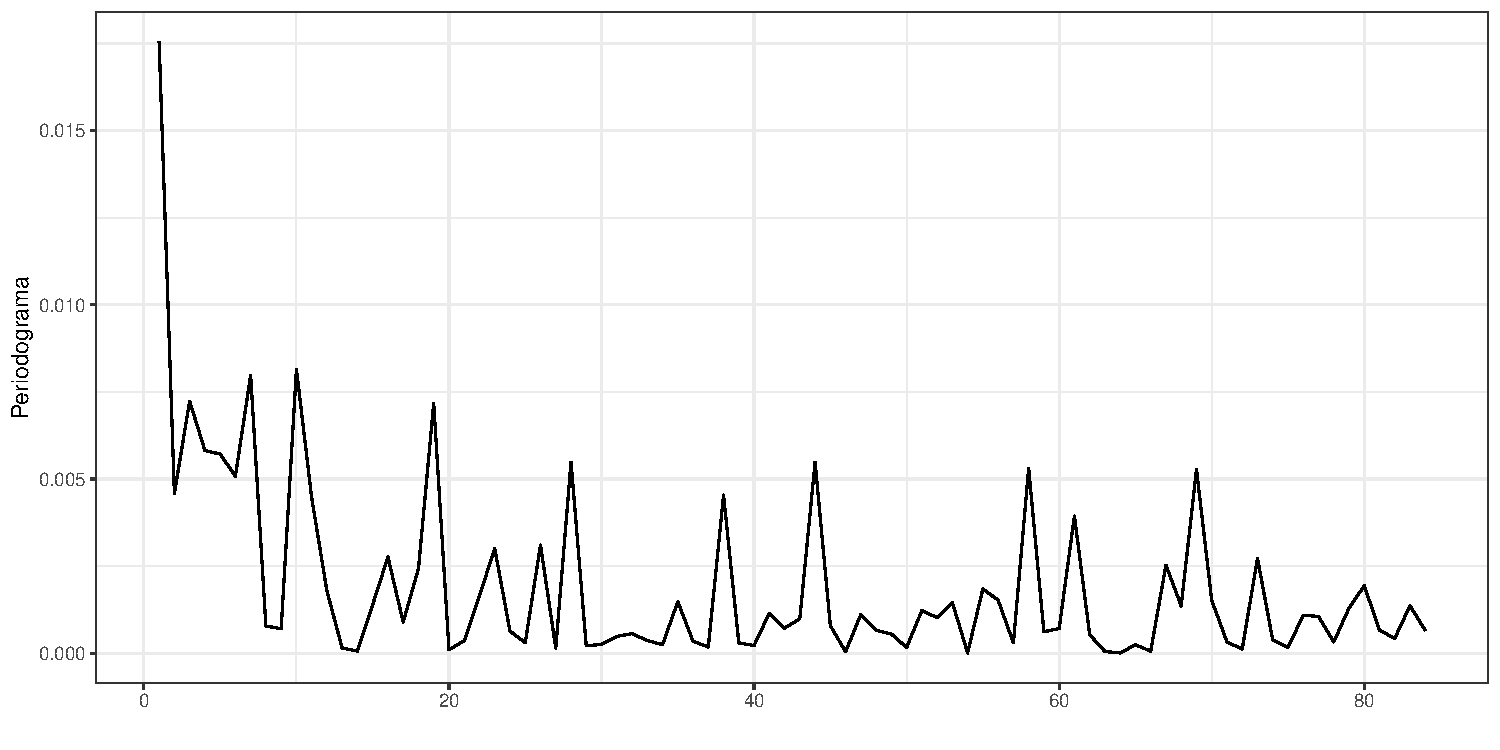
\includegraphics{pdf_tarea2_files/figure-pdf/fig-exp10-2.pdf}

}

\caption{\label{fig-exp10-2}Densidad espectral vs Periodograma}

\end{figure}



\end{document}
